\chapter{METODOLOGI}
\label{chap:metodologi}

\section{Metode yang dirancang}
\label{sec:metode yang dirancang}

Metode yang dirancang pada penelitian ini sebagaimana ditunjukkan pada Gambar \ref{fig:metode}

\begin{figure}[H]
  \centering
  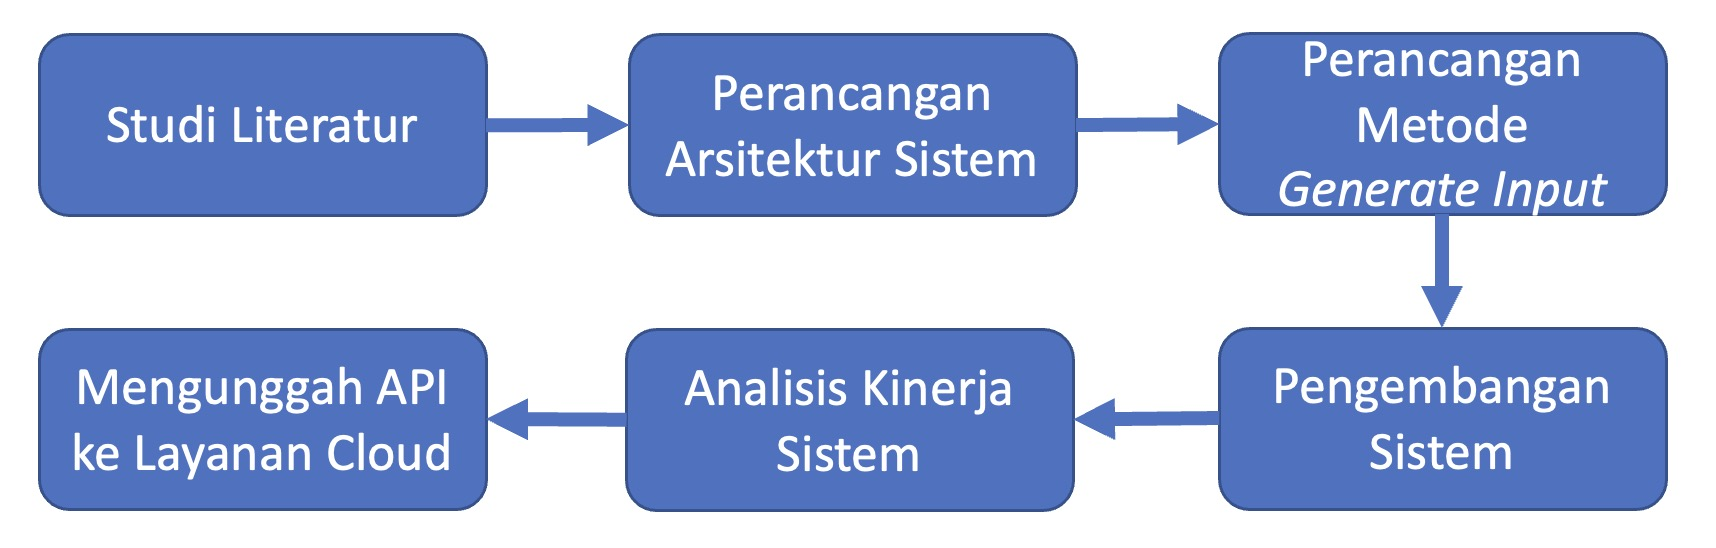
\includegraphics[scale=0.26]{gambar/DiagramAlirMetodePenelitian.jpg}

  % Ubah dengan keterangan gambar yang diinginkan
  \caption{Diagram Alir Metode Penelitian}
  \label{fig:metode}
\end{figure}
% what else except nolistsep?

\subsection{Studi Literatur}
\label{subsec:studiliteratur}

% \begin{itemize}[topsep=0pt]
  % \item \textbf{Studi Literatur}
  
  Pada tahap ini dilakukan riset studi literatur mengenai konsep 
  dan permasalahan - permasalahan yang sudah ada terkait DISC, 
  Apache Spark, Titian, DistilGPT2, dan FastAPI. Studi literatur didapatkan melalui buku, internet, jurnal penelitian, dan materi-materi kuliah yang berkaitan dengan metode yang akan digunakan.

  % \item \textbf{Perancangan Arsitektur Sistem}
  \subsection{Perancangan Arsitektur Sistem}
  \label{subsec:perancanganarsitektursistem}
  
  % Tahap perancangan arsitektur sistem pada penelitian ini 
  % dilakukan dengan mengombinasikan dasar teori dan penelitian 
  % terkait pada Bab \ref{chap:tinjauanpustaka}. 
  % Perancangan metode akan dimulai dari proses \emph{pre-training}
  % terhadap model DistilGPT2 menggunakan baris dataset random dari 
  % dataset masing-masing \emph{benchmark program} yang akan 
  % diuji. Kemudian program tersebut akan diberikan parameter tertentu 
  % agar dapat menghasilkan output yang bermasalah.
  % Dengan menggunakan Titian, akan dilakukan proses \emph{provenance data}
  % untuk mendapatkan nilai awal dari baris dataset yang menyebabkan
  % keluaran yang mencurigakan tersebut. 
  % Dilakukan proses re-training lagi terhadap
  % model DistilGPT2 menggunakan baris dataset penyebab kesalahan
  % tersebut yang kemudian dilakukan proses \emph{generate input}
  % baru yang menginduksi kesalahan pada program tersebut dengan jumlah
  % yang seminimal mungkin dapat dianalisis oleh \emph{developer}. 
  % Hasil dari proses ini kemudian akan dijalankan kembali menggunakan
  % program yang sama untuk melihat apakah program tersebut masih
  % menghasilkan keluaran yang bermasalah atau tidak.
  Tahap perancangan arsitektur sistem pada penelitian 
  ini dilakukan dengan mengombinasikan dasar teori dan 
  penelitian terkait pada Bab \ref{chap:tinjauanpustaka}. 
  Proses perancangan metode ini dijelaskan secara visual 
  dalam Gambar \ref{fig:arsitektur}. 
  Proses ini dibagi menjadi tiga fase utama:
  \begin{enumerate}[topsep=0pt]
    \item \textbf{Mengidentifikasi \emph{Faulty Input}}
    
    Proses ini dimulai dengan menggunakan Titian untuk 
    melakukan \emph{provenance data}. Tujuannya adalah 
    untuk mendapatkan nilai awal dari baris dataset 
    yang menyebabkan keluaran yang mencurigakan. 
    Program tersebut akan diberikan parameter 
    tertentu agar dapat menghasilkan output yang 
    bermasalah. Titian akan melacak asal-usul data 
    yang berkontribusi pada terjadinya kesalahan 
    dalam output, membantu dalam mengidentifikasi 
    sumber data yang menyebabkan masalah tersebut. 
    
    Dengan pemahaman yang lebih mendalam tentang 
    asal-usul data yang bermasalah, penelitian ini 
    dapat menetapkan dasar yang kuat untuk 
    langkah-langkah perbaikan berikutnya. Selain 
    itu, proses ini akan membantu memastikan bahwa 
    model memahami konteks dari kesalahan yang 
    terjadi, sehingga memungkinkan perbaikan yang 
    lebih tepat sasaran. Penelitian ini tidak akan 
    mempertimbangkan faktor struktur dari data, 
    sehingga memungkinkan untuk digunakan pada 
    banyak aplikasi. Dengan demikian, analisis 
    ini memberikan wawasan yang lebih mendalam 
    tentang bagaimana model berinteraksi dengan 
    data yang beragam dan menambah fleksibilitas 
    penggunaannya dalam berbagai konteks aplikasi.

    \item \textbf{Memproduksi \emph{Faulty Input} Baru} 
    
    Setelah proses \emph{provenance data} selesai, 
    langkah berikutnya adalah melakukan 
    \emph{pre-training} terhadap model DistilGPT2 
    menggunakan baris dataset random dari dataset 
    masing-masing \emph{benchmark program} yang 
    akan diuji. Langkah ini sangat penting untuk 
    memastikan bahwa model DistilGPT2 memiliki 
    dasar yang kuat dalam memahami pola umum dalam 
    data sebelum difokuskan pada data yang menyebabkan 
    kesalahan. Setelah itu, dilakukan proses 
    \emph{re-training} lagi terhadap model 
    DistilGPT2 menggunakan baris dataset penyebab 
    kesalahan tersebut. 
    
    Proses \emph{re-training} ini 
    dirancang untuk memperbaiki dan mengoptimalkan 
    model dengan memberikan perhatian khusus pada 
    data yang menyebabkan masalah, memastikan bahwa 
    model mampu mengenali dan mengatasi kesalahan 
    yang sama di masa depan. Kemudian dilakukan 
    proses \emph{generate input} baru yang menginduksi 
    kesalahan pada program tersebut dengan jumlah yang 
    seminimal mungkin dapat dianalisis oleh 
    \emph{developer}. Proses ini memungkinkan 
    pengembang untuk menguji program dengan input 
    baru yang dihasilkan oleh model, dan kemudian 
    secara manual menganalisis output untuk menemukan 
    sumber masalah.

    \item \textbf{Mengevaluasi Kemiripan Karakteristik 
    \emph{Faulty Input} Awal dengan \emph{Faulty Input} 
    Baru}

    Untuk menguji keefektifan model, hasil dari proses 
    ini kemudian akan dijalankan kembali menggunakan 
    program yang sama untuk melihat apakah program 
    tersebut masih menghasilkan keluaran yang bermasalah 
    atau tidak. Evaluasi kemiripan dilakukan dengan 
    membandingkan karakteristik data dari 
    \emph{faulty input} awal dengan \emph{faulty input}
    baru yang dihasilkan oleh model. Proses ini 
    bertujuan untuk memastikan bahwa input baru 
    yang dihasilkan oleh model memiliki kemiripan 
    yang relevan dengan data kesalahan yang ada 
    pada data awal. Dengan cara ini, penelitian 
    dapat menilai sejauh mana model berhasil dalam 
    mereplikasi kesalahan yang ada pada data asli 
    dan bagaimana efektifitasnya dalam menghasilkan 
    \emph{faulty input} yang serupa.

  \end{enumerate}

  % Perancangan metode akan dimulai dengan menggunakan 
  % Titian untuk melakukan proses \emph{provenance data}. 
  % Proses ini bertujuan untuk mendapatkan nilai awal dari 
  % baris dataset yang menyebabkan keluaran yang 
  % mencurigakan tersebut. Program tersebut akan 
  % diberikan parameter tertentu agar dapat menghasilkan 
  % output yang bermasalah. Titian akan melacak asal-usul 
  % data yang berkontribusi pada terjadinya kesalahan 
  % dalam output, membantu dalam mengidentifikasi sumber 
  % data yang menyebabkan masalah tersebut. Dengan 
  % pemahaman yang lebih mendalam tentang asal-usul 
  % data yang bermasalah, penelitian ini dapat menetapkan 
  % dasar yang kuat untuk langkah-langkah perbaikan 
  % berikutnya. Selain itu, proses ini akan membantu 
  % memastikan bahwa model memahami konteks dari 
  % kesalahan yang terjadi, sehingga memungkinkan 
  % perbaikan yang lebih tepat sasaran. Penelitian 
  % ini tidak akan mempertimbangkan faktor struktur 
  % dari data, sehingga memungkinkan untuk digunakan 
  % pada banyak aplikasi. Dengan demikian, analisis 
  % ini memberikan wawasan yang lebih mendalam tentang 
  % bagaimana model berinteraksi dengan data yang 
  % beragam dan menambah fleksibilitas penggunaannya 
  % dalam berbagai konteks aplikasi.
  
  % Setelah proses \emph{provenance data} selesai, 
  % langkah berikutnya adalah melakukan \emph{pre-training} 
  % terhadap model DistilGPT2 menggunakan baris dataset 
  % random dari dataset masing-masing 
  % \emph{benchmark program} yang akan diuji. 
  % Langkah ini sangat penting untuk memastikan bahwa 
  % model DistilGPT2 memiliki dasar yang kuat dalam 
  % memahami pola umum dalam data sebelum difokuskan 
  % pada data yang menyebabkan kesalahan. Setelah itu, 
  % dilakukan proses re-training lagi terhadap model 
  % DistilGPT2 menggunakan baris dataset penyebab 
  % kesalahan tersebut. Proses re-training ini 
  % dirancang untuk memperbaiki dan mengoptimalkan 
  % model dengan memberikan perhatian khusus pada 
  % data yang menyebabkan masalah, memastikan bahwa 
  % model mampu mengenali dan mengatasi kesalahan 
  % yang sama di masa depan. Kemudian dilakukan 
  % proses \emph{generate input} baru yang menginduksi 
  % kesalahan pada program tersebut dengan jumlah yang 
  % seminimal mungkin dapat dianalisis oleh 
  % \emph{developer}. Proses ini memungkinkan 
  % pengembang untuk menguji program dengan input 
  % baru yang dihasilkan oleh model, dan kemudian 
  % secara manual menganalisis output untuk menemukan 
  % sumber masalah. Untuk menguji keefektifan model,
  % hasil dari proses ini kemudian akan dijalankan
  % kembali menggunakan program yang sama untuk
  % melihat apakah program tersebut masih
  % menghasilkan keluaran yang bermasalah atau tidak. 
  % Hasil tersebut akan menunjukkan kemiripan dari 
  % karakteristik data yang dihasilkan oleh model
  % dengan data yang menyebabkan kesalahan pada program.
  % Alur keseluruhan proses tersebut dapat dilihat pada 
  % Gambar \ref{fig:arsitektur}.


  % Tahap perancangan arsitektur sistem pada penelitian ini 
  % dilakukan dengan mengombinasikan dasar teori dan penelitian 
  % terkait pada Bab \ref{chap:tinjauanpustaka}. 
  % Perancangan metode akan dimulai dari proses \emph{pre-training}
  % terhadap model DistilGPT2 menggunakan baris dataset random dari 
  % dataset masing-masing \emph{benchmark program} yang akan 
  % diuji. Kemudian program tersebut akan diberikan parameter tertentu 
  % agar dapat menghasilkan output yang bermasalah.
  % Dengan menggunakan Titian, akan dilakukan proses \emph{provenance data}
  % untuk mendapatkan nilai awal dari baris dataset yang menyebabkan
  % keluaran yang mencurigakan tersebut. 
  % Dilakukan proses re-training lagi terhadap
  % model DistilGPT2 menggunakan baris dataset penyebab kesalahan
  % tersebut yang kemudian dilakukan proses \emph{generate input}
  % baru yang menginduksi kesalahan pada program tersebut dengan jumlah
  % yang seminimal mungkin dapat dianalisis oleh \emph{developer}. 
  % Hasil dari proses ini kemudian akan dijalankan kembali menggunakan
  % program yang sama untuk melihat apakah program tersebut masih
  % menghasilkan keluaran yang bermasalah atau tidak.
  % Alur keseluruhan proses tersebut dapat dilihat pada 
  % Gambar \ref{fig:arsitektur}.


  

  % Bahas tentang perubahan data dari structured ke unstructured sebanyak satu paragraf

  Pada saat FISUM ditanamkan pada aplikasi DISC, 
  data yang dihasilkan oleh Titian berupa data 
  \emph{structured} yang terdiri dari beberapa kolom. 
  Namun, data yang dihasilkan oleh Titian harus
  diubah terlebih dahulu menjadi data \emph{unstructured}
  yang dapat diterima oleh model DistilGPT2.
  Hal ini dilakukan dengan cara menggabungkan
  kolom-kolom data tersebut menggunakan pemisah
  tertentu, dalam hal ini menggunakan ",".
  Setelah data tersebut diubah, baris data tersebut
  digabungkan menjadi satu baris utuh dengan pemisah "\#\#\#",
  sebelum dikirim melalui API yang
  kemudian diberikan ke model DistilGPT2 untuk
  dilatih kembali dan menghasilkan \emph{faulty input}
  baru yang dapat digunakan untuk membantu analis
  dalam melakukan analisis kesalahan pada aplikasi DISC.
  
  Data yang dihasilkan oleh model DistilGPT2 tersebut
  pada awalnya berupa data \emph{unstructured} yang
  kemudian diubah kembali menjadi data \emph{structured}
  untuk dapat dijalankan kembali pada aplikasi DISC.
  Alur perubahan data dari \emph{structured} ke \emph{unstructured}
  dan sebaliknya dapat dilihat pada gambar \ref{fig:AlurPerubahanData}.
  Warna merah pada dataset yang ditunjukkan oleh gambar
  tersebut menunjukkan data yang menginduksi kesalahan.

  \begin{figure}[H]
    \centering
    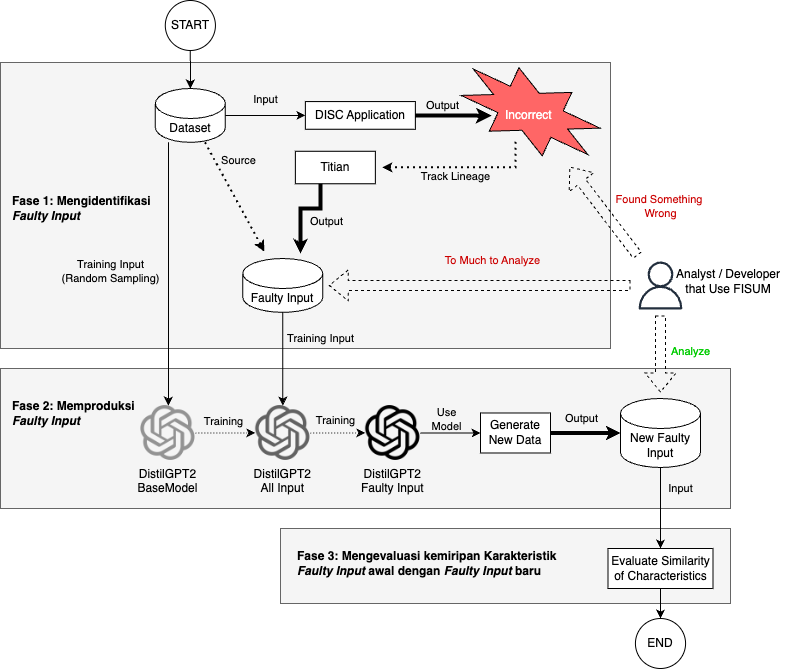
\includegraphics[scale=0.45]{gambar/ArsitekturFISUM.png}
  
    % Ubah dengan keterangan gambar yang diinginkan
    \caption{Rancangan Arsitektur Sistem}
    \label{fig:arsitektur}
  \end{figure}

  \begin{figure}[H]
    \centering
    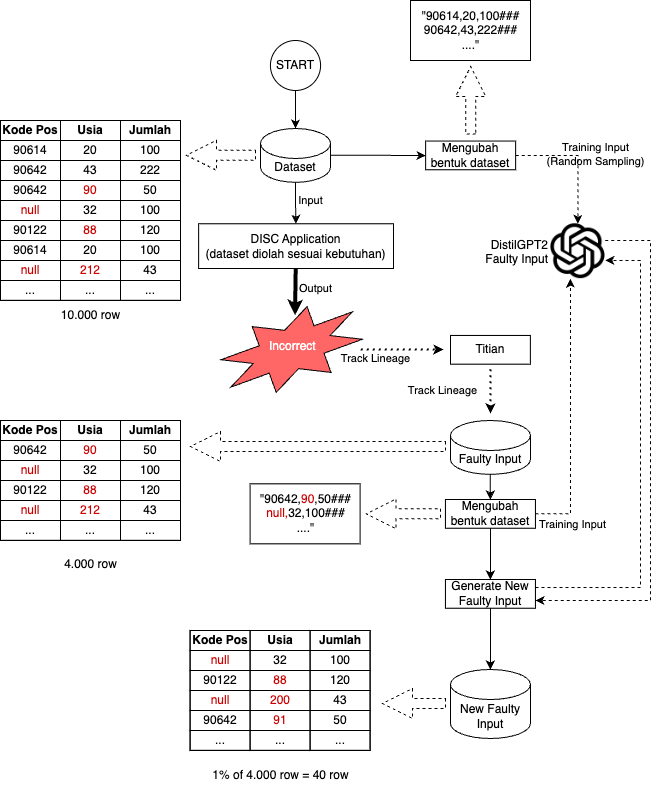
\includegraphics[scale=0.4]{gambar/AlurPerubahanData.png}
  
    % Ubah dengan keterangan gambar yang diinginkan
    \caption{Alur Perubahan Data}
    \label{fig:AlurPerubahanData}

  \end{figure}




  % \item \textbf{Perancangan Metode Generate Input}

  % \subsection{Perancangan Metode \emph{Generate Input}}

  % Tahap perancangan metode generate input dilakukan dengan 
  % melakukan proses traning dan re-training terhadap 
  % DistilGPT2 model yang memiliki \emph{hyperparameter} seperti
  % pada Tabel \ref{tab:hyperparameter}.
  % Proses ini dilakukan dengan membuat sebuah
  % API dengan menggunakan FastAPI yang dapat diakses oleh pengguna. 
  % API ini akan memiliki beberapa endpoint yang dapat digunakan 
  % oleh pengguna untuk melakukan proses \emph{generate input} baru, 
  % \emph{re-training new model}, dan \emph{reset model}. Proses 
  % penggunaan API ini dilakukan dalam dua tahap, yaitu \emph{local} 
  % dan \emph{cloud} milik Amazon Web Service (AWS).
  % Tahap ini dapat ditunjukkan melalui Gambar \ref{fig:generateinput}.

  \subsection{Perancangan Metode \emph{Generate Input}}
  \label{subsec:perancanganmetodegenerateinput}

Tahap perancangan metode \emph{generate input} dilakukan dengan 
melakukan proses training dan re-training terhadap model DistilGPT2 
yang memiliki \emph{hyperparameter} seperti pada Tabel \ref{tab:hyperparameter}. 
Proses ini dilakukan dengan membuat sebuah API menggunakan FastAPI 
yang dapat diakses oleh pengguna. API ini akan memiliki beberapa 
endpoint yang dapat digunakan oleh pengguna untuk melakukan proses 
\emph{generate input} baru, \emph{re-training new model}, dan \emph{reset model}. 
Proses penggunaan API ini dilakukan dalam dua tahap, yaitu \emph{local} dengan 
Uvicorn 
dan \emph{cloud} milik Amazon Web Service (AWS). 


\begin{table}[H]
  \centering
  \caption{Tabel \emph{hyperparameter} model DistilGPT2}
  \begin{tabular}{|p{0.25\linewidth}|p{0.25\linewidth}|}
    \hline
    \textbf{Hyperparameter} & \textbf{Nilai} \\
    \hline
    \raggedright \texttt{learning\_rate} & 5e-4 \\
    \hline
    \raggedright \texttt{warmup\_steps} & 1e2 \\
    \hline
    \raggedright \texttt{epsilon} & 1e-8 \\
    \hline
    \raggedright \texttt{batch\_size} & 2 \\
    \hline
    \raggedright \texttt{epochs} & 10 \\
    \hline
  \end{tabular}
  
  \label{tab:hyperparameter}
\end{table}


\begin{figure}[H]
  \centering
  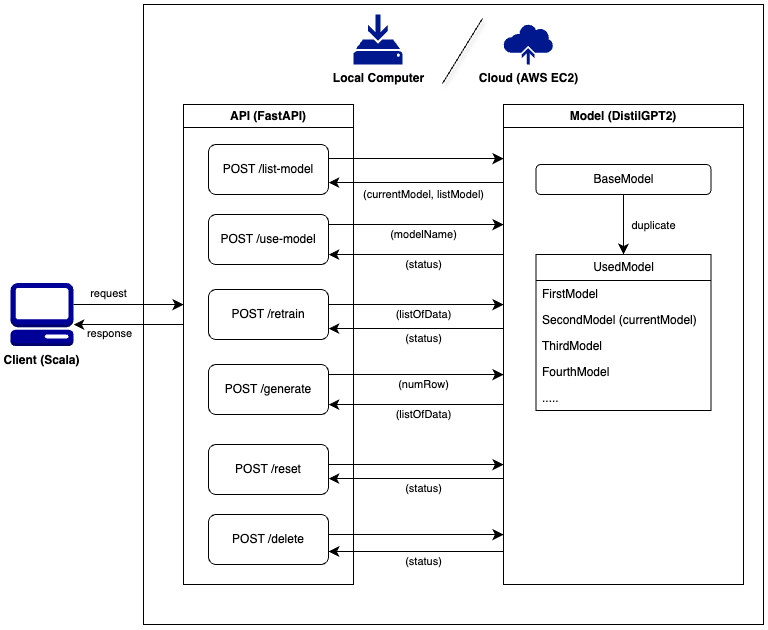
\includegraphics[scale=0.6]{gambar/RancanganMetodeGenerateInput.png}

  % Ubah dengan keterangan gambar yang diinginkan
  \caption{Rancangan Metode Generate Input}
  \label{fig:generateinput}

\end{figure}


\begin{table}[H]
  \centering
  \caption{Tabel API}
  \begin{tabular}{|p{0.18\linewidth}|p{0.25\linewidth}|p{0.17\linewidth}|p{0.28\linewidth}|}
    \hline
    \textbf{API} & \textbf{Deskripsi} & \textbf{Request Value}  & \textbf{Response Value} \\
    \hline
    \raggedright \texttt{POST /list-model} &\raggedright Menampilkan model yang terpakai dan tersedia & - &  current\_model, model\_list \\
    \hline
    \raggedright \texttt{POST /use-model} &\raggedright Mengganti model yang terpakai & model\_name & status \\
    \hline
    \texttt{POST /retrain} &\raggedright Melatih ulang model & dataset & status \\
    \hline
    \raggedright \texttt{POST /generate} &\raggedright Menghasilkan input yang menginduksi kesalahan & num\_row & list\_of\_generated\_row \\
    \hline
    \texttt{POST /reset} &\raggedright Mengembalikan model ke model dasar & - & status \\
    \hline
    \texttt{POST /delete} &\raggedright Menghapus model yang terpakai & - & status \\
    \hline
  \end{tabular}
  \label{tab:api}
\end{table}

API yang dikembangkan akan terdiri dari enam endpoint utama, masing-masing 
dengan fungsi spesifik untuk memudahkan pengguna dalam mengelola model 
DistilGPT2 dan proses \emph{generate input} yang ditunjukkan pada 
gambar \ref{fig:generateinput} dan tabel \ref{tab:api}.
Berikut adalah penjelasan lebih 
detail tentang setiap endpoint tersebut:

\begin{enumerate}[topsep=0pt, itemsep=0pt]
    \item \textbf{list-model}\\
    Endpoint ini mengembalikan daftar nama model yang tersedia. Pengguna dapat menggunakan endpoint ini untuk melihat model mana saja yang tersedia dan dapat digunakan. Ini membantu dalam pengelolaan model dengan memberikan informasi mengenai model yang telah di-deploy dan siap digunakan.
    
    \item \textbf{use-model}\\
    Endpoint ini digunakan untuk mengubah model yang sedang digunakan. Jika model yang diminta tidak ada dalam daftar, sistem akan membuat model baru dari model dasar. Endpoint ini berguna untuk pengembang yang ingin berpindah antara berbagai model atau membuat model baru berdasarkan kebutuhan spesifik mereka.
    
    \item \textbf{retrain}\\
    Endpoint ini digunakan untuk melakukan re-training terhadap model yang sedang digunakan. Proses re-training penting untuk memperbarui model dengan data baru atau memperbaiki performa model berdasarkan umpan balik terbaru. Endpoint ini memungkinkan pengembang untuk terus mengoptimalkan model agar tetap relevan dan akurat.
    
    \item \textbf{generate}\\
    Endpoint ini digunakan untuk menghasilkan input baru menggunakan model yang sedang digunakan. Endpoint ini memungkinkan pengguna untuk menghasilkan teks atau data baru yang dihasilkan oleh model DistilGPT2. Ini sangat berguna dalam aplikasi yang membutuhkan pembuatan teks otomatis atau analisis data.
    
    \item \textbf{reset}\\
    Endpoint ini digunakan untuk mengatur ulang model yang sedang digunakan ke kondisi dasar. Proses reset ini penting untuk mengembalikan model ke keadaan awal sebelum dilakukan re-training atau modifikasi lainnya. Ini berguna ketika pengembang perlu menghapus perubahan dan memulai kembali dari model dasar.
    
    \item \textbf{delete}\\
    Endpoint ini digunakan untuk menghapus model yang sedang digunakan. Penghapusan model diperlukan ketika model sudah tidak lagi dibutuhkan atau untuk membersihkan ruang penyimpanan. Endpoint ini memberikan fleksibilitas kepada pengembang untuk mengelola dan menghapus model sesuai kebutuhan.
\end{enumerate}

Setiap endpoint di atas memberikan fungsionalitas yang diperlukan untuk 
mengelola model DistilGPT2 secara efisien dan fleksibel, baik dalam lingkungan 
lokal Uvicorn maupun di cloud AWS.
  
  % \item \textbf{Pengembangan Sistem}\\
  \subsection{Pengembangan Sistem}
  \label{subsec:pengembangansistem}
  Pengembangan sistem dilakukan dengan menerapkan algoritma solusi yang dirancang dalam subbab perancangan arsitektur sistem dan perancangan metode generate input. Algoritma tersebut mencakup langkah-langkah yang terperinci untuk membangun dan mengelola sistem, serta memastikan bahwa semua komponen berfungsi dengan baik sesuai dengan tujuan penelitian. Pada tahap ini, penekanan diberikan pada integrasi antara berbagai komponen sistem dan pemanfaatan metode yang dirancang untuk menghasilkan input yang dapat memicu kesalahan dalam program yang diuji.

  Untuk API yang dikembangkan dalam perancangan metode generate input, bahasa pemrograman Python digunakan. Python dipilih karena kemampuannya dalam menangani berbagai operasi API dengan efisien dan mendukung pengembangan yang cepat. API ini menyediakan beberapa endpoint yang memungkinkan pengguna untuk melakukan berbagai operasi, termasuk membuat model baru, melakukan re-training, dan menghasilkan input baru. Endpoint ini diatur sedemikian rupa untuk mempermudah interaksi dengan model dan proses generate input melalui pemrograman berbasis Python.

  Sistem secara keseluruhan dibangun menggunakan bahasa pemrograman Scala, yang me-nawarkan kelebihan dalam hal kinerja dan dukungan untuk pemrosesan data besar. Setiap \emph{benchmark program} yang telah diatur parameternya dan ditanamkan dengan \emph{provenance engine} Titian akan membuat model baru pada server menggunakan FastAPI. FastAPI, yang dibangun dengan Python, digunakan untuk menangani pembuatan dan pengelolaan model secara efisien. Setelah model baru dibuat, proses \emph{re-training} dan \emph{generate input} baru dilakukan melalui API yang telah disediakan, memastikan bahwa semua langkah-langkah dalam sistem berfungsi secara sinergis.

  % \item \textbf{Analisis Kinerja Sistem}\\
  \subsection{Analisis Kinerja Sistem}
  \label{subsec:analisiskinerjasistem}
  Analisis kinerja sistem melibatkan evaluasi mendalam terhadap tiga aspek utama yang terkait dengan kemampuan sistem dalam mengelola dan memproses \emph{faulty input}. Pertama, fokus utama adalah mengidentifikasi \emph{faulty input} dengan menggunakan Titian. Pada tahap ini, akurasi sistem diuji dengan membandingkan jumlah dataset yang telah ditentukan sebagai \emph{faulty input} sebelumnya dengan jumlah dataset yang berhasil diidentifikasi oleh Titian. Hal ini penting untuk memastikan bahwa Titian dapat dengan efektif mendeteksi dan mengidentifikasi kesalahan dalam dataset yang diuji.

  Kedua, memproduksi \emph{faulty input} baru mencakup beberapa parameter kinerja penting. Waktu yang dibutuhkan untuk proses training model dan untuk menghasilkan \emph{faulty input} baru diukur guna menilai efisiensi sistem. Selain itu, akurasi dari \emph{faulty input} baru saat dijalankan ulang pada aplikasi DISC yang telah ditanamkan Titian juga diuji. Ini memastikan bahwa \emph{faulty input} baru yang dihasilkan relevan dan efektif dalam mengidentifikasi masalah pada aplikasi yang diuji.

  Ketiga, mengevaluasi kemiripan karakteristik \emph{faulty input} awal dengan \emph{faulty input} baru adalah langkah krusial dalam analisis kinerja. Perbandingan dilakukan dengan menggunakan Mean Squared Error (\emph{MSE}) untuk menilai kesamaan karakteristik data antara \emph{faulty input} awal dan yang baru dihasilkan oleh model. Evaluasi ini berfokus pada perbandingan jumlah tipe kesalahan untuk memastikan bahwa \emph{faulty input} baru memiliki karakteristik yang serupa dengan yang awal. Dengan analisis ini, dapat diperoleh wawasan mengenai sejauh mana model mampu menghasilkan input yang konsisten dan relevan dengan kesalahan yang telah diidentifikasi sebelumnya.
  % Analisis kinerja sistem yang akan dilakukan pada penelitian 
  % ini ada dua, yaitu tingkat akurasi dan waktu yang dibutuhkan. 
  % Terdapat dua poin yang akan diuji pada bagian akurasi yaitu 
  % dilakukan dengan membandingkan hasil dari dataset yang tetap 
  % mempertahankan kesalahan atau tidak, dan berapa persentase
  % jumlah dataset yang berhasil digenerate oleh model untuk
  % mereproduksi kesalahan tersebut. Sedangkan pada bagian waktu
  % yang dibutuhkan, dilakukan dengan menghitung waktu yang
  % dibutuhkan untuk menghasilkan sejumlah dataset yang bermasalah 
  % tersebut, dan berapa persentase waktu yang dibutuhkan untuk
  % melakukan \emph{re-training} model pada dataset tersebut.

  % \item \textbf{Mengunggah API ke Layanan \emph{Cloud}}\\
  \subsection{Mengunggah API ke Layanan \emph{Cloud}}
  \label{subsec:mengunggahapikelayanancloud}
  Setelah model telah berhasil dilatih untuk menghasilkan 
  input yang menginduksi kesalahan dan diuji untuk memastikan 
  efektivitasnya, langkah selanjutnya adalah mengunggah 
  \emph{API} ke layanan \emph{cloud}. Mengunggah \emph{API} 
  ke layanan \emph{cloud} memungkinkan akses yang mudah dan 
  skalabilitas untuk pengguna di berbagai lokasi. Dengan 
  menggunakan \emph{API} yang diunggah ke \emph{cloud}, 
  pengembang dapat mengotomatisasi proses deteksi dan 
  reproduksi kesalahan tanpa perlu mengelola infrastruktur 
  secara langsung. Layanan \emph{cloud} juga menyediakan 
  sumber daya yang diperlukan untuk menangani permintaan 
  \emph{API} dalam jumlah besar, memastikan bahwa alat 
  tetap responsif dan efisien bahkan di bawah beban kerja 
  yang tinggi. Langkah ini melibatkan konfigurasi server 
  \emph{cloud} untuk menjalankan \emph{LLM} dan mengatur 
  \emph{endpoint API} untuk menerima dan memproses permintaan 
  dari pengguna, memungkinkan integrasi yang mulus dengan 
  berbagai sistem dan aplikasi.

% \end{itemize}

\section{Peralatan Pendukung}
\label{sec:peralatan pendukung}

Terdapat beberapa peralatan hardware dan software pendukung yang digunakan untuk pengembangan sistem pada Tugas Akhir ini yang dapat dilihat sebagai berikut:
\begin{itemize}[topsep=0pt]
  \item Hardware
  \begin{enumerate}[topsep=0pt]
    \item Laptop MacBook Pro M2 2022
    \begin{enumerate}[topsep=0pt]
      \item Prosesor: Apple M2
      \item RAM: 8 GB
      \item Storage: 512 GB
      \item GPU: Apple M2
      \item OS: macOS Sonoma
    \end{enumerate}
  \end{enumerate}
  \item Software
  \begin{enumerate}[topsep=0pt]
    \item Google Colaboratory\\
    Digunakan untuk melakukan pelatihan model \emph{DistilGPT2}
    \item Visual Studio Code\\
    Digunakan untuk melakukan pengembangan program FastAPI
    \item IntelliJ IDEA CE\\
    Digunakan untuk melakukan pengembangan program Scala
    \item HuggingFace\\
    Digunakan untuk mengakses model \emph{DistilGPT2}
    \item Amazon Web Service EC2\\
    Digunakan untuk melakukan \emph{deployment} 
    API ke \emph{cloud}
  \end{enumerate}
  \item Sumber Dana
  \begin{enumerate}[topsep=0pt]
    \item LPDP\\  
    Pendaan berasal dari Direktorat Jenderal Pendidikan Tinggi,
    Kementerian Pendidikan, Kebudayaan, Riset, dan Teknologi
    melalui beasiswa \emph{research} Garuda ACE
  \end{enumerate}
\end{itemize}
\section{Implementasi}
\label{sec:implementasi}
Tujuan utama dari penelitian ini adalah menghasilkan data 
yang menyebabkan kesalahan dalam jumlah yang dapat dengan 
mudah dianalisis oleh developer. 
Gambar \ref{fig:arsitektur2} merangkum alur 
kerja penelitian ini. 

\begin{figure}[H]
  \centering
  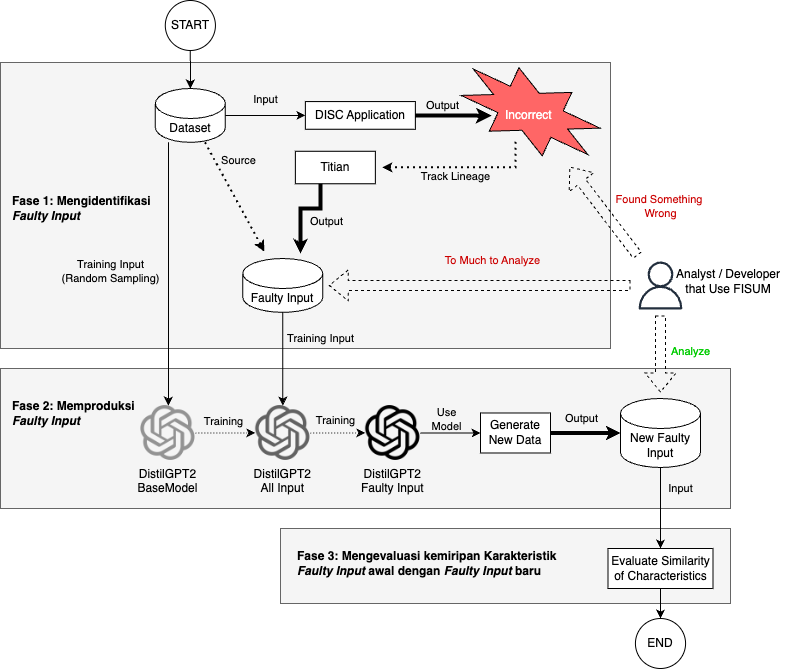
\includegraphics[scale=0.5]{gambar/ArsitekturFISUM.png}

  % Ubah dengan keterangan gambar yang diinginkan
  \caption{Rancangan Arsitektur Sistem}
  \label{fig:arsitektur2}
\end{figure}

Berikut adalah fase-fase implementasi yang dilakukan dalam
penelitian ini:

\subsection{Mengidentifikasi \emph{Faulty Input}}
\label{sec:mengidentifikasifaultyinput}

Pada fase ini, sistem FISUM mengidentifikasi data 
yang menyebabkan keluaran yang mencurigakan atau 
kesalahan pada sistem DISC. Alur kerja penggunaan Titian pada \emph{benchmark program}
dapat dilihat pada Gambar \ref{fig:diagramofprogramwithtitian}.

\begin{figure}[H]
  \centering
  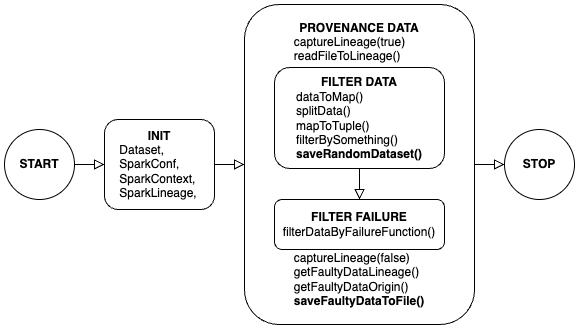
\includegraphics[scale=0.5]{gambar/DiagramOfProgramWithTitian.png}

  % Ubah dengan keterangan gambar yang diinginkan
  \caption{Diagram Alur Kerja Program dengan Titian}
  \label{fig:diagramofprogramwithtitian}
\end{figure}

\begin{enumerate}[topsep=0pt, itemsep=0pt]
  \item \textbf{Integrasi dengan Titian:}
  \begin{itemize}
      \item \textbf{Setup Titian:} Pastikan Titian terintegrasi dengan sistem DISC, sehingga Titian dapat diakses untuk melacak data.
      Langkah untuk mempersiapkan Titian dapat dilihat pada point-point berikut:
      \begin{enumerate}[topsep=0pt]
        \item \textbf{Unduh \emph{Library} Titian:} Unduh Titian dari repositori Spark dan ekstrak ke direktori yang diinginkan. Versi Titian yang digunakan adalah spark-2.1.1-SNAPSHOT-bin-titian-2.1.
        \item \textbf{Masukkan \emph{File} Jar:} Masukkan file jar Titian ke dalam proyek Scala dengan cara membuka \emph{project structure}, SDKs, \emph{classpath}, dan pilih semua 
        \emph{file} jar Titian yang diperlukan dari dalam \emph{folder} jars Titian. Proses tersebut dapat dilihat
        pada Gambar \ref{fig:masukkanfilejar}.

        \begin{figure}[H]
          \centering
          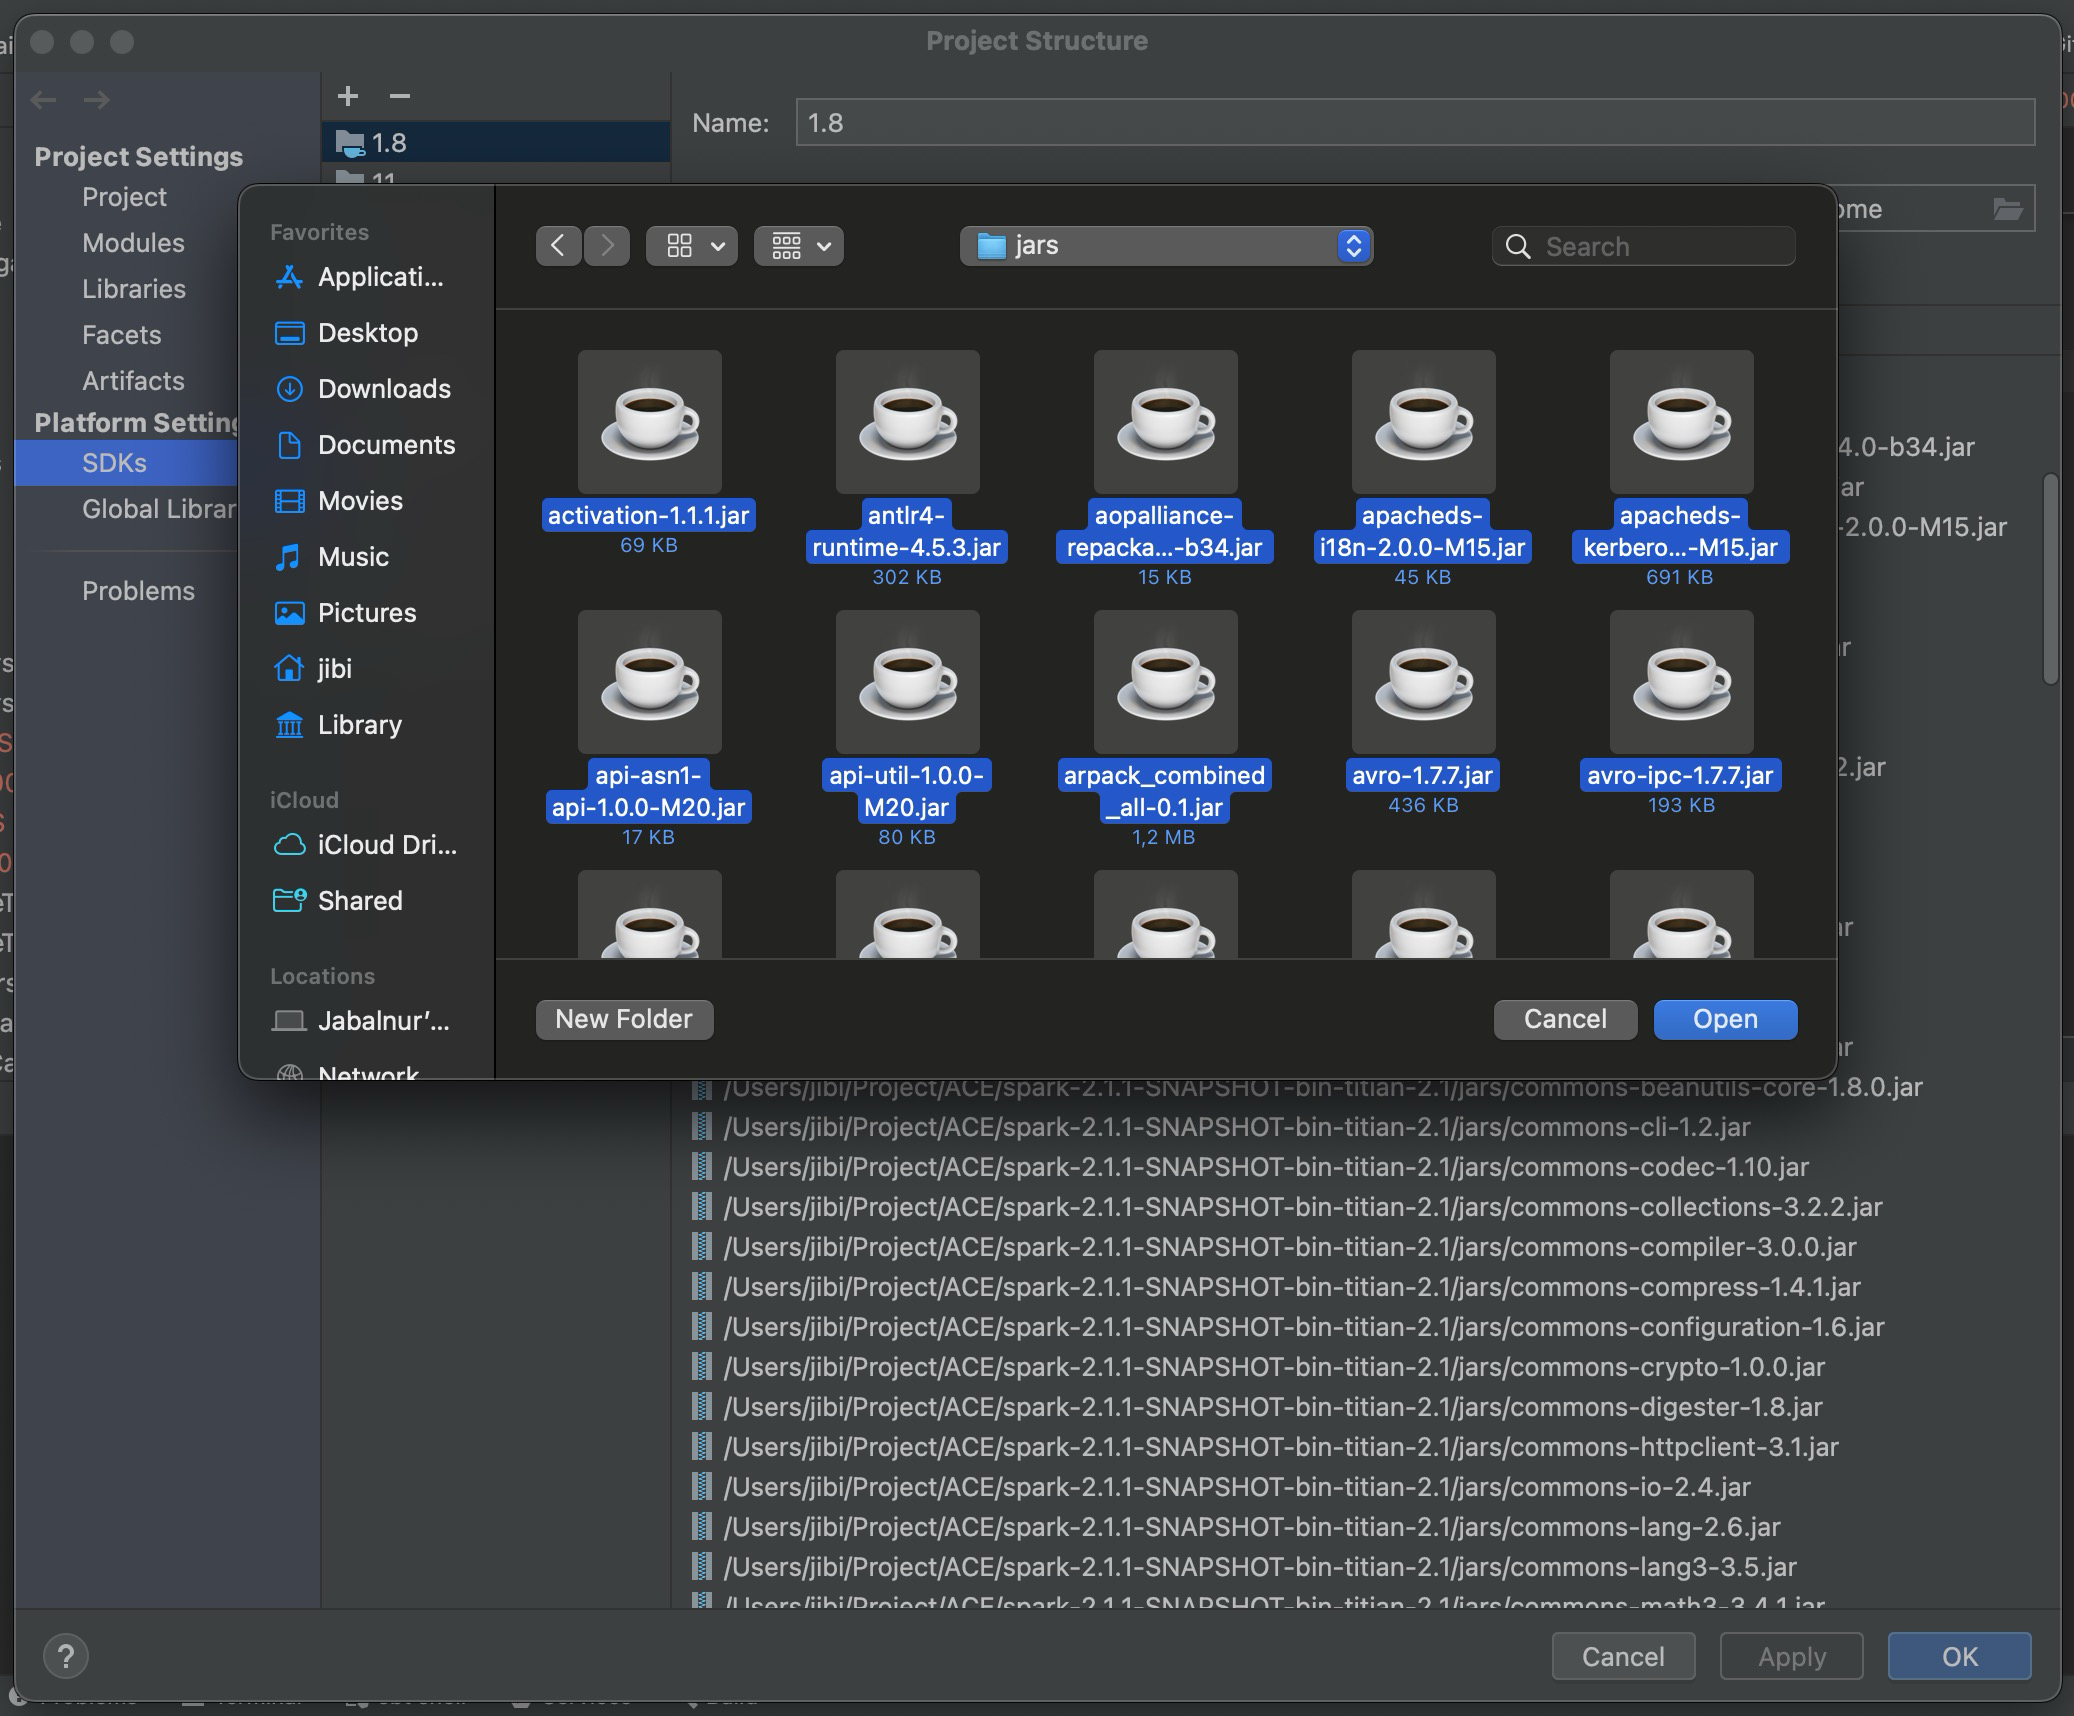
\includegraphics[scale=0.16]{gambar/MasukkanFileJar.png}
        
          % Ubah dengan keterangan gambar yang diinginkan
          \caption{Masukkan \emph{File} Jar}
          \label{fig:masukkanfilejar}
        \end{figure}
      \end{enumerate}
      \item \textbf{Pengaturan Titian:} Konfigurasikan Titian untuk melacak data yang berkontribusi pada keluaran yang mencurigakan, mengidentifikasi bagian dari data yang menyebabkan kesalahan.
      Kode untuk mengatur Titian untuk melacak data dapat dilihat pada Kode Sumber \ref{lst:settinguptitian}.

      \lstinputlisting[
        language=Scala,
        caption={Pengaturan Titian},
        label={lst:settinguptitian},
        captionpos=b
      ]{program/scala/titian/setting-up-titian-pseu.scala}

      Potongan Kode Sumber \ref{lst:settinguptitian} dimulai dengan membuat objek \texttt{SparkConf} bernama \texttt{conf} untuk konfigurasi Spark. Variabel \texttt{lineage} diatur ke \texttt{true} untuk \emph{lineage tracking}. File sumber data ditetapkan dengan \texttt{logFile = "src/dataset.csv"}. Konfigurasi \texttt{conf} diatur untuk menjalankan Spark dalam mode \emph{local} dengan satu thread melalui \texttt{setMaster("local[1]")}. Kemudian, objek \texttt{SparkContext} dibuat menggunakan \texttt{conf}, dan objek \texttt{LineageContext} dibuat dari \texttt{SparkContext} (\texttt{sc}) untuk \emph{lineage tracking}.


  \end{itemize}


  
  
  \item \textbf{\emph{Provenance Data} dengan Scala:}
  \begin{itemize}

    \item \textbf{Lacak \emph{Lineage} Data:} Gunakan Titian untuk melacak provenance data dari keluaran yang bermasalah ke data input yang menyebabkan kesalahan.
    Kode untuk melacak provenance data menggunakan Titian dapat dilihat pada Kode Sumber \ref{lst:trackprovenancedata}.

    \lstinputlisting[
      language=Scala,
      caption={Lacak Provenance Data},
      label={lst:trackprovenancedata},
      captionpos=b
    ]{program/scala/titian/track-provenance-data-pseu.scala}

    Pada Kode Sumber \ref{lst:trackprovenancedata}, \texttt{lc.setCaptureLineage(true)} digunakan untuk mengaktifkan \emph{lineage capture} sebelum menjalankan aplikasi \emph{DISC}. Kode aplikasi \emph{DISC} ditempatkan di antara dua pemanggilan \texttt{setCaptureLineage}, yang memungkinkan pelacakan semua operasi yang dilakukan selama eksekusi aplikasi tersebut. Setelah aplikasi \emph{DISC} selesai dijalankan, \texttt{lc.setCaptureLineage(false)} dipanggil untuk menonaktifkan \emph{lineage capture}.


      \item \textbf{Pengambilan Data:} Ambil dataset dari sistem DISC yang berkontribusi pada keluaran yang mencurigakan.
      Kode untuk mengambil data dari Titian dapat dilihat pada Kode Sumber \ref{lst:getdatafromtitian}.

      \lstinputlisting[
        language=Scala,
        caption={Ambil Data dari Titian},
        label={lst:getdatafromtitian},
        captionpos=b
      ]{program/scala/titian/get-data-from-titian-pseu.scala}

      Pada Kode Sumber \ref{lst:getdatafromtitian}, \texttt{var linRdd = mapped2.getLineage()} digunakan untuk mendapatkan \emph{lineage} dari \texttt{mapped2} dan menyimpannya dalam variabel \texttt{linRdd}. Kemudian, \texttt{linRdd = linRdd.goBackAll()} dipanggil untuk mengembalikan \emph{lineage} ke tahap awal dari semua operasi yang telah dilakukan, sehingga dapat melacak kembali semua transformasi yang terjadi. 
      
      Terakhir, \texttt{linRdd.show.saveAsTextFile("src/output/faulty-data")} digunakan untuk menampilkan dan menyimpan hasil \emph{lineage} dalam bentuk file teks di direktori \texttt{"src/output/faulty-data"}, yang berisi data yang diidentifikasi sebagai \emph{faulty}.
      \\
      \\

  \end{itemize}
\end{enumerate}

\subsection{Memproduksi \emph{Faulty Input} Baru}
\label{sec:memproduksifaultyinput}
\begin{enumerate}[topsep=0pt]
  \item \textbf{Setup FastAPI:}
  \begin{itemize}
      \item \textbf{Pengembangan API:} Kembangkan API menggunakan FastAPI yang menerima data unstructure dari aplikasi Scala, dan melakukan training atau re-training model DistilGPT2, dan menghasilkan \emph{faulty input} baru.
      Kode Sumber \ref{lst:fastapi} menunjukkan kode untuk mengembangkan API menggunakan FastAPI.

      \lstinputlisting[
        language=Python,
        caption={Pengembangan API FastAPI},
        label={lst:fastapi},
        captionpos=b
      ]{program/python/api.py}

      Kode Sumber \ref{lst:fastapi} mendefinisikan sebuah aplikasi \emph{FastAPI} yang menyediakan beberapa \emph{endpoints} untuk berinteraksi dengan model \emph{DistilGPT2}. Pada bagian awal, modul-modul yang diperlukan diimpor, termasuk \texttt{FastAPI} dan \texttt{Depends} dari \texttt{fastapi}, serta \texttt{BaseModel} dari \texttt{pydantic}. Kemudian, objek \texttt{app} dibuat sebagai \emph{instance} dari \emph{FastAPI}.

      \begin{itemize}
        \item \texttt{@app.post("/retrain")} \\
        mendefinisikan \emph{endpoint} untuk melatih ulang model dengan teks baru yang diberikan melalui \texttt{GenericRetrainRequest}.
        \item \texttt{@app.post("/generate")} \\
        mendefinisikan \emph{endpoint} untuk menghasilkan teks baru berdasarkan jumlah teks yang diminta dalam \texttt{GenericGenerateRequest}. Hasilnya dikembalikan sebagai \texttt{GenericGenerateResponse}.
        \item \texttt{@app.post("/reset")} \\
        mendefinisikan \emph{endpoint} untuk mereset model ke status awal. Status reset dikembalikan sebagai \texttt{GenericResetResponse}.
        \item \texttt{@app.post("/delete")} \\
        mendefinisikan \emph{endpoint} untuk menghapus model. Status penghapusan dikembalikan sebagai \texttt{GenericDeleteResponse}.
        \item \texttt{@app.post("/model-list")} \\
        mendefinisikan \emph{endpoint} untuk mendapatkan daftar model yang tersedia dan model yang sedang digunakan.
        \item \texttt{@app.post("/use-model")} \\
        mendefinisikan \emph{endpoint} untuk memilih model tertentu yang akan digunakan. Status pemilihan model dikembalikan sebagai \texttt{GenericUseModelResponse}.
      \end{itemize}


      \item \textbf{Melihat List Model DistilGPT2 yang Tersedia:} Lihat model DistilGPT2 yang tersedia dan yang sedang digunakan untuk \emph{training} atau \emph{re-training}, dan \emph{generate} input baru.
      Kode untuk melihat list model DistilGPT2 yang tersedia dapat dilihat pada Kode Sumber \ref{lst:listmodel}.

      \lstinputlisting[
        language=Python,
        caption={List Model DistilGPT2},
        label={lst:listmodel},
        captionpos=b
      ]{program/python/list-model.py}

      Kode Sumber \ref{lst:listmodel} mendefinisikan dua baris yang berfungsi untuk mendapatkan daftar model dari direktori yang ditentukan dan mengembalikannya bersama dengan model yang sedang digunakan. 
      
      Pertama, \texttt{self.model\_list = get\_dir\_list(config["USED\_DIR"])} digunakan untuk mendapatkan daftar model yang tersedia di direktori yang ditentukan oleh \emph{konfigurasi} \texttt{config["USED\_DIR"]} dan menyimpannya dalam \texttt{self.model\_list}. Kemudian, \texttt{return self.current\_model, self.model\_list} mengembalikan model yang sedang digunakan (\texttt{self.current\_model}) dan daftar model yang tersedia (\texttt{self.model\_list}) sebagai hasil.

      \item \textbf{Memilih Model DistilGPT2 sesuai dengan \emph{Benchmark Program}:} Pilih model DistilGPT2 yang sesuai dengan \emph{benchmark program} yang akan diuji.
      Kode untuk memilih model DistilGPT2 dapat dilihat pada Kode Sumber \ref{lst:selectmodel}.

      \lstinputlisting[
        language=Python,
        caption={Pilih Model DistilGPT2},
        label={lst:selectmodel},
        captionpos=b
      ]{program/python/select-model.py}

      Kode sumber yang ditunjukkan dalam \ref{lst:selectmodel} mendefinisikan berbagai parameter penting yang diperlukan untuk melatih model \emph{DistilGPT2} dan menginisialisasi model tersebut dengan \emph{tokenizer} serta \emph{optimizer}. 
      \\

      Pada baris 1 hingga 7, parameter \emph{hyperparameter} diatur, meliputi \texttt{learning\_rate} untuk menentukan kecepatan pembelajaran model, \texttt{warmup\_steps} yang mengatur jumlah langkah pemanasan sebelum \emph{learning rate} mencapai nilai maksimalnya, \texttt{epsilon} untuk stabilitas numerik dalam perhitungan, \texttt{batch\_size} yang menentukan ukuran batch data untuk pelatihan, \texttt{epochs} untuk jumlah iterasi pelatihan penuh melalui dataset, \texttt{sample\_every} yang menentukan frekuensi sampling data selama pelatihan, dan \texttt{seed\_val} yang digunakan untuk memastikan hasil pelatihan yang dapat direproduksi.
      \\

      Langkah berikutnya adalah mendapatkan daftar model yang tersedia di direktori yang ditentukan oleh konfigurasi \texttt{config["USED\_DIR"]}. Ini dilakukan pada baris 9 dengan menggunakan fungsi \texttt{get\_dir\_list}, yang mengembalikan daftar nama model dalam direktori tersebut dan menyimpannya dalam \texttt{self.model\_list}. Setelah itu, model yang digunakan diatur dengan \texttt{self.current\_model = model} pada baris 10. Apabila model yang ditentukan tidak ada dalam daftar model yang tersedia, program akan mencetak pesan kesalahan dan menyalin file model dasar dari direktori konfigurasi ke direktori yang digunakan pada baris 12 hingga 14.
      \\

      Selanjutnya, \texttt{self.tokenizer} diinisialisasi menggunakan \texttt{GPT2Tokenizer} pada baris 17 dengan model \emph{DistilGPT2}, serta token awal (\texttt{bos\_token}), token akhir (\texttt{eos\_token}), dan token pengisi (\texttt{pad\_token}) yang ditetapkan ke string kosong. Inisialisasi ini penting untuk memastikan tokenizer yang digunakan sesuai dengan model yang dimuat.
      \\

      Konfigurasi model kemudian diatur menggunakan \texttt{GPT2Config.from\_pretrained} pada baris 19, yang memuat konfigurasi model dari file konfigurasi yang ada di direktori yang digunakan, dengan opsi untuk tidak menyimpan \emph{hidden states}. Pada baris 21, model \texttt{self.model} diinisialisasi menggunakan \texttt{GPT2LMHeadModel} dengan file model yang telah dilatih sebelumnya dan konfigurasi yang ditentukan. 
      \\

      Untuk menyesuaikan ukuran \emph{token embeddings} model agar sesuai dengan ukuran \texttt{tokenizer}, digunakan \texttt{self.model.resize\_token\_embeddings()} pada baris 23. Optimizer diatur menggunakan \texttt{torch.optim.AdamW} pada baris 25 hingga 28, dengan parameter model, \emph{learning rate}, dan \emph{epsilon} yang telah ditentukan.
      \\

      Terakhir, model dan perangkat (\emph{device}) diatur untuk menggunakan GPU jika tersedia; jika tidak, CPU akan digunakan. Hal ini dilakukan pada baris 30 hingga 35 dengan memeriksa ketersediaan CUDA dan mengatur model serta perangkat yang sesuai. Untuk memastikan bahwa hasil pelatihan dapat direproduksi, digunakan kode pada baris 37 hingga 40.
      \\
      % \item \textbf{Setup DistilGPT2:} Setup model DistilGPT2 
      % milik HuggingFace untuk melakukan \emph{training} 
      % atau \emph{re-training} model.
      % Kode untuk setup model DistilGPT2 dapat dilihat pada Kode Sumber \ref{lst:setupdistilgpt2}.

      % \lstinputlisting[
      %   language=Python,
      %   caption={Setup Model DistilGPT2},
      %   label={lst:setupdistilgpt2},
      %   captionpos=b
      % ]{program/python/setup-distilgpt2.py}

      \item \textbf{Setup Training Model:} Persiapkan data dan konfigurasi model DistilGPT2 untuk \emph{training} atau \emph{re-training}. Pastikan data sudah diproses sesuai format yang diinginkan dan atur hyperparameter seperti \emph{learning rate} dan ukuran \emph{batch}. Kode untuk setup \emph{training} model DistilGPT2 dapat dilihat pada Kode Sumber \ref{lst:setuptrainingdistilgpt2}.
      \\
      \\
      \\

      \lstinputlisting[
        language=Python,
        caption={Setup Training Model DistilGPT2},
        label={lst:setuptrainingdistilgpt2},
        captionpos=b
      ]{program/python/setup-training-distilgpt2.py}

      Kode Sumber \ref{lst:setuptrainingdistilgpt2} bertujuan untuk memproses dataset, menginisialisasi tokenizer, dan menyiapkan data untuk pelatihan model \emph{DistilGPT2}. 
      Pertama, dataset dipecah menjadi beberapa bagian berdasarkan separator \texttt{"\#\#\#"} menggunakan metode \texttt{split} pada baris 1. Hasil pemecahan ini disimpan dalam variabel \texttt{texts}, yang kemudian dikonversi menjadi objek \texttt{pandas.Series} pada baris 2. Ini memungkinkan penggunaan fitur-fitur dari \texttt{pandas} untuk analisis data lebih lanjut jika diperlukan.
      \\

      Pada baris 4 hingga 11, tokenizer diinisialisasi dan dua list kosong, \texttt{self.input\_ids} dan \texttt{self.attn\_masks}, disiapkan untuk menyimpan ID token dan masker perhatian yang akan dihasilkan. Untuk setiap teks dalam \texttt{txt\_list}, teks tersebut diproses oleh tokenizer untuk menghasilkan ID token dan masker perhatian. Fungsi \texttt{tokenizer} digunakan dengan parameter \texttt{truncation=True} untuk memotong teks yang lebih panjang dari \texttt{max\_length}, dan \texttt{padding="max\_length"} untuk memastikan semua teks memiliki panjang yang konsisten. Hasilnya adalah kamus (\texttt{dict}) yang berisi \texttt{input\_ids} dan \texttt{attention\_mask}, yang kemudian diubah menjadi tensor PyTorch dan ditambahkan ke list masing-masing.
      \\

      Setelah semua teks diproses, \texttt{dataset} diatur menjadi tuple yang terdiri dari dua variabel yaitu \texttt{self.input\_ids} dan \texttt{self.attn\_masks}. Pada baris 14 hingga 16, dataset dibagi menjadi dataset pelatihan dan validasi. Ukuran dataset pelatihan ditentukan sebagai 90\% dari total dataset, sementara ukuran dataset validasi adalah sisa dari dataset. Fungsi \texttt{random\_split} dari PyTorch digunakan untuk membagi dataset dengan proporsi yang ditentukan.
      Pada baris 18 hingga 24, \texttt{DataLoader} diatur untuk dataset pelatihan dan validasi. \texttt{DataLoader} digunakan untuk memuat data secara batch selama pelatihan. Untuk dataset pelatihan, \texttt{RandomSampler} digunakan untuk memastikan bahwa data diambil secara acak. Untuk dataset validasi, \texttt{SequentialSampler} digunakan untuk memastikan bahwa data diproses dalam urutan yang konsisten. Parameter \texttt{batch\_size} ditentukan sesuai dengan nilai yang telah diatur sebelumnya.
      \\

      Baris 26 hingga 31 berfungsi untuk mengatur jadwal pelatihan dengan menggunakan fungsi \texttt{get\_linear\_schedule\_with\_warmup}. Fungsi ini membuat jadwal \emph{learning rate} yang memulai dengan nilai kecil, meningkat secara linear selama \texttt{num\_warmup\_steps}, dan kemudian menurun hingga akhir pelatihan. Total langkah pelatihan dihitung berdasarkan ukuran \texttt{train\_dataloader} dan jumlah epoch yang ditentukan.
      \\

      Akhirnya, pada baris 33, waktu awal pelatihan dicatat dengan menggunakan fungsi \texttt{time.time()}, dan model dipindahkan ke perangkat yang sesuai (GPU atau CPU) menggunakan \texttt{self.model.to(self.device)}.
      \\

      \item \textbf{Training Model:} Latih model DistilGPT2 menggunakan data yang telah disiapkan dengan memulai proses pelatihan. Selama \emph{training}, model akan memproses data dalam beberapa iterasi (epochs), memperbarui parameter berdasarkan feedback dari fungsi kerugian untuk meningkatkan akurasi. Pastikan untuk memantau kinerja model dan menyesuaikan hyperparameter sesuai kebutuhan untuk mencapai hasil terbaik. Proses ini biasanya memanfaatkan perangkat keras seperti GPU untuk efisiensi. Kode untuk \emph{training} model DistilGPT2 dapat dilihat pada Kode Sumber \ref{lst:trainingdistilgpt2}.
      \\
      \\
      

      
      \lstinputlisting[
        language=Python,
        caption={Training Model DistilGPT2},
        label={lst:trainingdistilgpt2},
        captionpos=b
      ]{program/python/training-distilgpt2.py}

      Pada Kode Sumber \ref{lst:trainingdistilgpt2}, proses pelatihan model dilakukan dalam beberapa epoch yang ditentukan oleh \texttt{self.epochs}. Untuk setiap epoch, waktu mulai dicatat pada baris pertama.
      Di dalam loop epoch, \texttt{self.model.train()} mengatur model dalam mode pelatihan. Selanjutnya, untuk setiap batch dalam \texttt{train\_dataloader}, input, label, dan masker perhatian dipindahkan ke perangkat (GPU/CPU) yang sesuai. Model direset gradienya dengan \texttt{self.model.zero\_grad()}.
      \\

      Model kemudian dipanggil dengan \texttt{b\_input\_ids}, \texttt{b\_labels}, dan \texttt{b\_masks} untuk mendapatkan output dan menghitung kerugian (\texttt{loss}). Kerugian per batch dijumlahkan untuk menghitung \texttt{total\_train\_loss}. Setelah itu, \texttt{loss.backward()} akan menghitung gradien, dan \texttt{self.optimizer.step()} memperbarui bobot model. Jadwal pelatihan diperbarui dengan \texttt{scheduler.step()}.
      Akhirnya, rata-rata kerugian pelatihan dihitung dengan membagi \texttt{total\_train\_loss} dengan jumlah batch.
      \\
      \\

      \item \textbf{Generate Input:} Hasilkan \emph{faulty input} baru yang menginduksi kesalahan menggunakan model DistilGPT2 yang telah dilatih.
      Kode untuk menghasilkan \emph{faulty input} baru dapat dilihat pada Kode Sumber \ref{lst:generateinput}.

      \lstinputlisting[
        language=Python,
        caption={Generate Input},
        label={lst:generateinput},
        captionpos=b
      ]{program/python/generate-input.py}

      Pada Kode Sumber \ref{lst:generateinput}, pertama-tama, program memeriksa apakah model yang saat ini dipilih adalah "none" pada baris pertama. Jika demikian, akan mengembalikan pesan kesalahan yang menunjukkan bahwa tidak ada model yang dipilih dan meminta pengguna untuk memilih model dari daftar yang tersedia.
      Jika model yang saat ini dipilih valid, program melanjutkan dengan mengatur model ke mode evaluasi dengan \texttt{self.model.eval()} pada baris 2. Ini memastikan bahwa model berfungsi dalam mode evaluasi, di mana beberapa mekanisme seperti dropout dinonaktifkan.
      Selanjutnya, prompt kosong diinisialisasi dan diubah menjadi tensor dengan menggunakan tokenizer pada baris 4 hingga 6. Tensor ini kemudian dipindahkan ke perangkat yang sesuai (GPU/CPU) dengan \texttt{to(self.device)}.
      \\

      \texttt{self.model.generate()} digunakan untuk menghasilkan teks berdasarkan prompt yang diberikan. Parameter \texttt{do\_sample=True} mengaktifkan sampling untuk menghasilkan teks yang lebih bervariasi. Parameter lain seperti \texttt{top\_k}, \texttt{max\_length}, \texttt{top\_p}, dan \texttt{num\_return\_sequences} mengatur bagaimana teks dihasilkan, termasuk panjang teks dan jumlah hasil yang dikembalikan.
      Setelah teks dihasilkan, setiap tensor output didekode menjadi string dengan \texttt{self.tokenizer.decode(n, skip\_special\_tokens=True)} pada baris 9 hingga 11. String-string ini kemudian digabungkan dengan separator "\#\#\#" untuk membentuk \texttt{data\_text}, yang kemudian dikembalikan sebagai hasil akhir.



      \item \textbf{Reset Model:} Kembalikan model DistilGPT2 ke kondisi awal sebelum \emph{training} atau \emph{re-training}.
      Hal ini dilakukan untuk membersihkan model dari data yang telah digunakan dan mempersiapkan model untuk \emph{training} atau \emph{re-training} selanjutnya.
      Kode untuk mereset model DistilGPT2 dapat dilihat pada Kode Sumber \ref{lst:resetmodel}.

      \lstinputlisting[
        language=Python,
        caption={Reset Model},
        label={lst:resetmodel},
        captionpos=b
      ]{program/python/reset-model.py}

      Kode Sumber \ref{lst:resetmodel} bertujuan untuk menyiapkan model \emph{DistilGPT2} dengan membersihkan dan menyalin file, serta menginisialisasi tokenizer, model, dan optimizer.
      Pertama, \texttt{make\_dir\_empty()} pada baris 1 digunakan untuk mengosongkan direktori yang ditentukan, yang merupakan direktori tempat model saat ini disimpan. Fungsi ini memastikan bahwa direktori tersebut bersih sebelum menyalin file baru ke dalamnya. Setelah itu, \texttt{copy\_files()} pada baris 2 menyalin file dari direktori \texttt{BASE\_DIR} ke direktori \texttt{USED\_DIR}, yang sekarang berisi model yang sedang digunakan.
      Selanjutnya, tokenizer diinisialisasi menggunakan \texttt{GPT2Tokenizer} pada baris 3, yang memuat tokenizer yang telah dilatih sebelumnya dengan model \emph{DistilGPT2}. Tokenizer ini dikonfigurasi dengan token awal, token akhir, dan token pengisi yang kosong.
      \\

      Konfigurasi model dimuat dengan \texttt{GPT2Config} pada baris 4, yang membaca file konfigurasi dari direktori model saat ini. Parameter \texttt{output\_hidden\_states=False} mengatur agar model tidak mengembalikan \emph{hidden states}.
      Model \texttt{GPT2LMHeadModel} diinisialisasi pada baris 5 dengan bobot yang telah dilatih sebelumnya yang disimpan dalam file \texttt{pytorch\_model.bin} dan konfigurasi yang telah dimuat.
      Pada baris 7, ukuran \emph{token embeddings} model disesuaikan agar sesuai dengan ukuran tokenizer yang baru. Optimizer diatur menggunakan \texttt{torch.optim.AdamW()} pada baris 8 hingga 10 dengan parameter \texttt{learning\_rate} dan \texttt{epsilon} yang telah ditentukan.

      Akhirnya, pada baris 12 hingga 16, perangkat keras untuk pelatihan ditentukan. Jika GPU tersedia, model dipindahkan ke GPU dengan \texttt{self.model.cuda()}. Jika tidak, model dipindahkan ke CPU dengan \texttt{self.model.to(self.device)}. 


      \item \textbf{Hapus Model:} Hapus model DistilGPT2 yang tidak diperlukan lagi.
      Hal ini dilakukan untuk membersihkan ruang penyimpanan dan mengelola model yang digunakan.
      Kode untuk menghapus model DistilGPT2 dapat dilihat pada Kode Sumber \ref{lst:deletemodel}.

      \lstinputlisting[
        language=Python,
        caption={Hapus Model},
        label={lst:deletemodel},
        captionpos=b
      ]{program/python/delete-model.py}

      Kode Sumber \ref{lst:deletemodel} digunakan untuk menghapus model yang sedang digunakan dan memperbarui daftar model yang tersedia.
      Pertama, \texttt{delete\_dir()} pada baris 1 menghapus direktori yang berisi model saat ini. Direktori yang dihapus ditentukan oleh \texttt{config["USED\_DIR"]} dan \texttt{self.current\_model}, yang mengacu pada lokasi penyimpanan model yang akan dihapus. Fungsi ini menghapus semua file dan subdirektori di dalam direktori tersebut, membersihkan ruang penyimpanan.
      Selanjutnya, \texttt{self.current\_model} diatur ke "none" pada baris 2. Ini menunjukkan bahwa tidak ada model yang sedang dipilih atau digunakan saat ini, dan sistem siap untuk memilih model lain di masa depan.
      Terakhir, \texttt{self.model\_list} diperbarui dengan memanggil \texttt{get\_dir\_list()} pada baris 3. Fungsi ini mengembalikan daftar model yang tersedia di direktori \texttt{config["USED\_DIR"]}, yang kemudian disimpan dalam \texttt{self.model\_list}. Dengan cara ini, daftar model yang tersedia selalu diperbarui untuk mencerminkan status terbaru sistem.

      \item \textbf{Deployment FastAPI:} Deploy API FastAPI ke server lokal atau cloud untuk memudahkan pengguna dalam mengakses dan menggunakan API.
      Kode untuk melakukan \emph{deployment} FastAPI dapat dilihat pada Kode Sumber \ref{lst:deploymentfastapi}.

      \lstinputlisting[
        caption={Deployment FastAPI},
        label={lst:deploymentfastapi},
        captionpos=b
      ]{program/deployment-fastapi.txt}

      Kode Sumber \ref{lst:deploymentfastapi} dimulai dengan mengatur direktori kerja ke \texttt{/app}. Setelah itu, file \texttt{Pipfile} disalin ke direktori tersebut dan \texttt{pipenv} diinstal untuk mengelola dependensi Python. Dependensi yang tercantum dalam \texttt{Pipfile} kemudian diinstal. Selanjutnya, lingkungan virtual diaktifkan, meskipun biasanya tidak diperlukan untuk otomatisasi. Akhirnya, \texttt{uvicorn} dijalankan untuk melayani aplikasi FastAPI yang terletak di modul \texttt{main} dengan objek \texttt{app}, yang memungkinkan akses aplikasi pada port 8000.


  \end{itemize}
  
  \item \textbf{Integrasi dengan Scala:}
  \begin{itemize}
      \item \textbf{Akses API dari Scala:} Buat panggilan HTTP untuk berinteraksi dengan API FastAPI dari aplikasi Scala.
      Kode untuk mengakses API FastAPI dari Scala dapat dilihat pada Kode Sumber \ref{lst:scala-api-pseudocode}.

      \lstinputlisting[
        caption={\emph{Pseudocode} penggunaan API pada Scala},
        label={lst:scala-api-pseudocode},
        captionpos=b
      ]{program/scala-api-pseudocode.txt}

      Kode Scala ini menggambarkan proses untuk mengakses API dan melakukan berbagai operasi terkait model dan data. Pertama, didefinisikan daftar persentase yang akan digunakan untuk menghasilkan data baru melalui \texttt{percentageOutput}. Proses dimulai dengan mengakses model menggunakan \texttt{useModelRequest()}; jika statusnya bukan \texttt{"Success"}, sistem akan dihentikan dengan \texttt{system.terminate()}. Selanjutnya, daftar model yang tersedia diambil melalui \texttt{getModelListRequest()}, yang mencakup model saat ini dan daftar model lainnya. 
      \\

      Data dari file \texttt{all\_data.csv} dikonversi menjadi daftar dan digunakan untuk retrain model dengan memilih data secara acak, yang kemudian digabungkan dengan pemisah "\#\#\#" dan dikirim melalui \texttt{retrainRequest()}. Status retrain diperiksa, dan jika tidak berhasil, sistem dihentikan. Data dari file \texttt{incorrect\_data.csv} juga digunakan untuk retrain model dengan cara yang sama. 
      \\
      
      Untuk menghasilkan data baru, kode menghitung jumlah baris data berdasarkan persentase dalam \texttt{percentageOutput}, lalu data baru dihasilkan dengan memanggil \texttt{generateInputRequest()} dan disimpan ke file yang sesuai. Opsional, model dapat di-reset dengan \texttt{resetModelRequest()} dan dihapus dengan menggunakan \texttt{deleteModelRequest()}; jika status operasi tersebut bukan \texttt{"Success"}, sistem dihentikan. Akhirnya, sistem dihentikan setelah semua operasi selesai dengan menjalankan \texttt{system.terminate()}.

      
  \end{itemize}
\end{enumerate}

\begin{itemize}
  \item \textbf{Konversi Data \emph{Structured} ke \emph{Unstructured}:} Gabungkan kolom data menggunakan separator "," untuk mempersiapkan data sebelum digunakan dalam model DistilGPT2.
  Agar dapat dikirim melalui API FastAPI, data kemudian diubah menjadi satu text utuh dengan
  menyatukan baris data menggunakan separator "\#\#\#".
  Proses konversi data dari \emph{structured} ke \emph{unstructured} dapat dilihat pada Kode Sumber \ref{lst:structuredtounstructured}.

  \lstinputlisting[
    language=Scala,
    caption={Konversi Data Structured ke Unstructured},
    label={lst:structuredtounstructured},
    captionpos=b
  ]{program/scala/structured-to-unstructured.scala}

  Kode Sumber \ref{lst:structuredtounstructured} melakukan beberapa langkah untuk memproses file dalam sebuah direktori. Pertama, objek \texttt{directory} dibuat dengan menentukan path direktori menggunakan \texttt{new File(dir)}. Kemudian, variabel \texttt{data} diinisialisasi dengan hasil dari pemeriksaan apakah direktori tersebut ada dan benar-benar sebuah direktori. Jika kondisi ini terpenuhi, maka \texttt{directory.listFiles()} digunakan untuk mendapatkan daftar semua file dalam direktori. Daftar ini kemudian difilter untuk menyertakan hanya file (bukan subdirektori), dan nama-nama file tersebut diambil dengan \texttt{\_.getName}. Daftar nama file yang didapat kemudian diubah menjadi list dengan \texttt{toList}. Jika direktori tidak ada atau bukan direktori, \texttt{data} diinisialisasi sebagai list kosong \texttt{List.empty[String]}.

  Setelah itu, variabel \texttt{data} yang berisi nama-nama file diubah menjadi sebuah string tunggal dengan memisahkan setiap nama file menggunakan pemisah \texttt{"\#\#\#"}. Proses ini dilakukan dengan menggunakan metode \texttt{mkString("\#\#\#")} yang menggabungkan semua elemen list menjadi satu string dengan pemisah yang ditentukan di antara elemen-elemen tersebut.


\end{itemize}

\subsection{Mengevaluasi Kemiripan Karakteristik 
\emph{Faulty Input} Awal dengan \emph{Faulty Input} Baru}
\label{sec:mengevaluasikemiripan}

Untuk mengevaluasi kemiripan antara \emph{faulty input} awal dan \emph{faulty input} baru yang dihasilkan oleh model DistilGPT2, dilakukan beberapa langkah penting. Evaluasi ini bertujuan untuk memastikan bahwa \emph{faulty input} baru efektif dalam mereplikasi kesalahan yang ada pada \emph{faulty input} awal dan untuk menilai akurasi serta kualitas dari \emph{faulty input} baru. Berikut adalah langkah-langkah yang dilakukan:

\begin{enumerate}[topsep=0pt]
    \item \textbf{Pengujian Akurasi:}
    Setelah \emph{faulty input} baru dihasilkan, langkah pertama adalah menjalankan data ini dalam aplikasi DISC yang sudah ditanamkan dengan Titian. Ini untuk memverifikasi apakah aplikasi DISC masih menghasilkan keluaran yang bermasalah saat diberikan \emph{faulty input} baru. Pengujian ini memastikan bahwa \emph{faulty input} baru benar-benar dapat mereplikasi kesalahan yang sama seperti \emph{faulty input} awal.
    Kode untuk memverifikasi akurasi \emph{faulty input} baru dapat dilihat pada Kode Sumber \ref{lst:verifyaccuracy}.

    \lstinputlisting[
      language=Scala,
      caption={Verifikasi Akurasi Faulty Input Baru},
      label={lst:verifyaccuracy},
      captionpos=b
    ]{program/scala/evaluasi/verify-accuracy.scala}

    Kode Sumber \ref{lst:verifyaccuracy} memproses data dari dua file CSV untuk mengidentifikasi baris data yang dianggap data "\emph{faulty}" atau "\emph{not faulty}". Pertama, file \texttt{incorrect\_data.csv} dan \texttt{incorrect\_data\_from\_titian.csv} dibaca dan dikonversi menjadi list string menggunakan fungsi \texttt{fileToList()}. Variabel \texttt{resultFISUM} akan menyimpan data dari file \texttt{incorrect\_data.csv}, sedangkan \texttt{resultFISUMFromTitian} menyimpan data dari file \texttt{incorrect\_data\_from\_titian.csv}.
    \\

    Sebuah array dua dimensi \texttt{result} diinisialisasi dengan ukuran \texttt{resultFISUM.length} x 2, untuk menyimpan hasil identifikasi. Untuk setiap baris dalam \texttt{resultFISUM}, kode memeriksa apakah baris tersebut juga terdapat dalam \texttt{resultFISUMFromTitian}. Jika baris ditemukan dalam \texttt{resultFISUMFromTitian}, maka baris tersebut ditandai sebagai "faulty" dan disimpan di \texttt{result} pada indeks yang sesuai. Jika tidak ditemukan, baris tersebut ditandai sebagai "not faulty". 
    Akhirnya, seluruh array \texttt{result} dicetak ke konsol menggunakan \texttt{result.foreach(println)}, menampilkan setiap baris data berserta statusnya.


    \item \textbf{Perhitungan MSE (Mean Squared Error):}
      Untuk mengukur kemiripan antara \emph{faulty input} awal dan \emph{faulty input} baru secara kuantitatif, kita menghitung Mean Squared Error (MSE) dari perbandingan karakteristik yang dimiliki kedua jenis \emph{faulty input}. MSE memberikan ukuran seberapa besar perbedaan antara karakteristik \emph{faulty input} yang dimiliki oleh kedua dataset tersebut.
      Kode untuk menghitung MSE antara \emph{faulty input} awal dan baru dapat dilihat pada Kode Sumber \ref{lst:calculatemse}.

      \lstinputlisting[
        language=Scala,
        caption={Perhitungan MSE},
        label={lst:calculatemse},
        captionpos=b
      ]{program/scala/evaluasi/calculate-mse.scala}

      Kode Sumber \ref{lst:calculatemse} bertujuan untuk menganalisis dan membandingkan data dari dua file CSV dan menghitung Mean Squared Error (MSE) antara hasil analisis dari kedua file. Pertama, variabel \texttt{result} diinisialisasi sebagai array dengan empat elemen yang bernilai nol. Data dari file \texttt{incorrect\_data.csv} dibaca dan dikonversi menjadi list string dengan \texttt{fileToList()}. Setiap baris data diproses dengan membaginya menggunakan koma sebagai pemisah.
      Baris-baris data yang memenuhi kondisi tertentu, yaitu kolom pertama bernilai "null" dan kolom kedua lebih dari 50, ditandai dengan menambahkan label "mid" dan meningkatkan elemen kedua dalam array \texttt{result}. Jika hanya kolom pertama bernilai "null", label "left" ditambahkan dan elemen pertama dalam array \texttt{result} ditingkatkan. Jika hanya kolom kedua lebih dari 50, label "right" ditambahkan dan elemen ketiga dalam array \texttt{result} ditingkatkan. 
      \\

      Setelah pemrosesan data, array \texttt{result} dinormalisasi dengan membagi setiap elemennya dengan nilai minimum dalam array \texttt{result}. Langkah serupa dilakukan untuk data dari file \texttt{new\_incorrect\_dataset\_2953.csv}, menghasilkan array \texttt{resultFisum} yang juga dinormalisasi dengan membagi setiap elemennya dengan nilai minimum dalam array \texttt{resultFisum}.
      Perbedaan kuadrat antara elemen-elemen array \texttt{result} dan \texttt{resultFisum} dihitung dan disimpan dalam array \texttt{differences}. Mean Squared Error (MSE) dihitung dengan menjumlahkan elemen-elemen dalam array \texttt{differences} dan membaginya dengan jumlah elemen array tersebut. Hasil MSE dicetak ke konsol.
      \\

\end{enumerate}


